%% bare_adv.tex
%% V1.4b
%% 2015/08/26
%% by Michael Shell
%% See: 
%% http://www.michaelshell.org/
%% for current contact information.
%%
%% This is a skeleton file demonstrating the advanced use of IEEEtran.cls
%% (requires IEEEtran.cls version 1.8b or later) with an IEEE Computer
%% Society journal paper.
%%
%% Support sites:
%% http://www.michaelshell.org/tex/ieeetran/
%% http://www.ctan.org/pkg/ieeetran
%% and
%% http://www.ieee.org/

%%*************************************************************************
%% Legal Notice:
%% This code is offered as-is without any warranty either expressed or
%% implied; without even the implied warranty of MERCHANTABILITY or
%% FITNESS FOR A PARTICULAR PURPOSE! 
%% User assumes all risk.
%% In no event shall the IEEE or any contributor to this code be liable for
%% any damages or losses, including, but not limited to, incidental,
%% consequential, or any other damages, resulting from the use or misuse
%% of any information contained here.
%%
%% All comments are the opinions of their respective authors and are not
%% necessarily endorsed by the IEEE.
%%
%% This work is distributed under the LaTeX Project Public License (LPPL)
%% ( http://www.latex-project.org/ ) version 1.3, and may be freely used,
%% distributed and modified. A copy of the LPPL, version 1.3, is included
%% in the base LaTeX documentation of all distributions of LaTeX released
%% 2003/12/01 or later.
%% Retain all contribution notices and credits.
%% ** Modified files should be clearly indicated as such, including  **
%% ** renaming them and changing author support contact information. **
%%*************************************************************************


% *** Authors should verify (and, if needed, correct) their LaTeX system  ***
% *** with the testflow diagnostic prior to trusting their LaTeX platform ***
% *** with production work. The IEEE's font choices and paper sizes can   ***
% *** trigger bugs that do not appear when using other class files.       ***                          ***
% The testflow support page is at:
% http://www.michaelshell.org/tex/testflow/


% IEEEtran V1.7 and later provides for these CLASSINPUT macros to allow the
% user to reprogram some IEEEtran.cls defaults if needed. These settings
% override the internal defaults of IEEEtran.cls regardless of which class
% options are used. Do not use these unless you have good reason to do so as
% they can result in nonIEEE compliant documents. User beware. ;)
%
%\newcommand{\CLASSINPUTbaselinestretch}{1.0} % baselinestretch
%\newcommand{\CLASSINPUTinnersidemargin}{1in} % inner side margin
%\newcommand{\CLASSINPUToutersidemargin}{1in} % outer side margin
%\newcommand{\CLASSINPUTtoptextmargin}{1in}   % top text margin
%\newcommand{\CLASSINPUTbottomtextmargin}{1in}% bottom text margin




%
\documentclass[10pt,journal,compsoc]{IEEEtran}
\usepackage{xeCJK}
\usepackage{diagbox}
% If IEEEtran.cls has not been installed into the LaTeX system files,
% manually specify the path to it like:
% \documentclass[10pt,journal,compsoc]{../sty/IEEEtran}


% For Computer Society journals, IEEEtran defaults to the use of 
% Palatino/Palladio as is done in IEEE Computer Society journals.
% To go back to Times Roman, you can use this code:
%\renewcommand{\rmdefault}{ptm}\selectfont





% Some very useful LaTeX packages include:
% (uncomment the ones you want to load)



% *** MISC UTILITY PACKAGES ***
%
%\usepackage{ifpdf}
% Heiko Oberdiek's ifpdf.sty is very useful if you need conditional
% compilation based on whether the output is pdf or dvi.
% usage:
% \ifpdf
%   % pdf code
% \else
%   % dvi code
% \fi
% The latest version of ifpdf.sty can be obtained from:
% http://www.ctan.org/pkg/ifpdf
% Also, note that IEEEtran.cls V1.7 and later provides a builtin
% \ifCLASSINFOpdf conditional that works the same way.
% When switching from latex to pdflatex and vice-versa, the compiler may
% have to be run twice to clear warning/error messages.




% *** CITATION PACKAGES ***
%
\ifCLASSOPTIONcompsoc
  % The IEEE Computer Society needs nocompress option
  % requires cite.sty v4.0 or later (November 2003)
  \usepackage[nocompress]{cite}
\else
  % normal IEEE
  \usepackage{cite}
\fi
% cite.sty was written by Donald Arseneau
% V1.6 and later of IEEEtran pre-defines the format of the cite.sty package
% \cite{} output to follow that of the IEEE. Loading the cite package will
% result in citation numbers being automatically sorted and properly
% "compressed/ranged". e.g., \cite{ShiZhongci2000}, \cite{QiuXipeng2020}, \cite{LuJinfu2004}, \cite{duraisamy2015}, \cite{kopriva2009}, \cite{wang2017} without using
% cite.sty will become \cite{ShiZhongci2000}, \cite{LuJinfu2004}, \cite{kopriva2009}--\cite{duraisamy2015}, \cite{QiuXipeng2020} using cite.sty. cite.sty's
% \cite will automatically add leading space, if needed. Use cite.sty's
% noadjust option (cite.sty V3.8 and later) if you want to turn this off
% such as if a citation ever needs to be enclosed in parenthesis.
% cite.sty is already installed on most LaTeX systems. Be sure and use
% version 5.0 (2009-03-20) and later if using hyperref.sty.
% The latest version can be obtained at:
% http://www.ctan.org/pkg/cite
% The documentation is contained in the cite.sty file itself.
%
% Note that some packages require special options to format as the Computer
% Society requires. In particular, Computer Society  papers do not use
% compressed citation ranges as is done in typical IEEE papers
% (e.g., \cite{ShiZhongci2000}-\cite{chapra1998}). Instead, they list every citation separately in order
% (e.g., \cite{ShiZhongci2000}, \cite{LuJinfu2004}, \cite{logan2014}, \cite{chapra1998}). To get the latter we need to load the cite
% package with the nocompress option which is supported by cite.sty v4.0
% and later.



\usepackage{graphics}

% *** GRAPHICS RELATED PACKAGES ***
%
\ifCLASSINFOpdf
   \usepackage[pdftex]{graphicx}
  % declare the path(s) where your graphic files are
  % \graphicspath{{../pdf/}{../jpeg/}}
  % and their extensions so you won't have to specify these with
  % every instance of \includegraphics
  % \DeclareGraphicsExtensions{.pdf,.jpeg,.png}
\else
  % or other class option (dvipsone, dvipdf, if not using dvips). graphicx
  % will default to the driver specified in the system graphics.cfg if no
  % driver is specified.
  \usepackage[dvips]{graphicx}
  % declare the path(s) where your graphic files are
  % \graphicspath{{../eps/}}
  % and their extensions so you won't have to specify these with
  % every instance of \includegraphics
  % \DeclareGraphicsExtensions{.eps}
\fi
% graphicx was written by David Carlisle and Sebastian Rahtz. It is
% required if you want graphics, photos, etc. graphicx.sty is already
% installed on most LaTeX systems. The latest version and documentation
% can be obtained at: 
% http://www.ctan.org/pkg/graphicx
% Another good source of documentation is "Using Imported Graphics in
% LaTeX2e" by Keith Reckdahl which can be found at:
% http://www.ctan.org/pkg/epslatex
%
% latex, and pdflatex in dvi mode, support graphics in encapsulated
% postscript (.eps) format. pdflatex in pdf mode supports graphics
% in .pdf, .jpeg, .png and .mps (metapost) formats. Users should ensure
% that all non-photo figures use a vector format (.eps, .pdf, .mps) and
% not a bitmapped formats (.jpeg, .png). The IEEE frowns on bitmapped formats
% which can result in "jaggedy"/blurry rendering of lines and letters as
% well as large increases in file sizes.
%
% You can find documentation about the pdfTeX application at:
% http://www.tug.org/applications/pdftex





% *** MATH PACKAGES ***

\usepackage{amsmath}
\usepackage{amssymb}
% A popular package from the American Mathematical Society that provides
% many useful and powerful commands for dealing with mathematics.
%
% Note that the amsmath package sets \interdisplaylinepenalty to 10000
% thus preventing page breaks from occurring within multiline equations. Use:
%\interdisplaylinepenalty=2500
% after loading amsmath to restore such page breaks as IEEEtran.cls normally
% does. amsmath.sty is already installed on most LaTeX systems. The latest
% version and documentation can be obtained at:
% http://www.ctan.org/pkg/amsmath





% *** SPECIALIZED LIST PACKAGES ***
%\usepackage{acronym}
% acronym.sty was written by Tobias Oetiker. This package provides tools for
% managing documents with large numbers of acronyms. (You don't *have* to
% use this package - unless you have a lot of acronyms, you may feel that
% such package management of them is bit of an overkill.)
% Do note that the acronym environment (which lists acronyms) will have a
% problem when used under IEEEtran.cls because acronym.sty relies on the
% description list environment - which IEEEtran.cls has customized for
% producing IEEE style lists. A workaround is to declared the longest
% label width via the IEEEtran.cls \IEEEiedlistdecl global control:
%
% \renewcommand{\IEEEiedlistdecl}{\IEEEsetlabelwidth{SONET}}
% \begin{acronym}
%
% \end{acronym}
% \renewcommand{\IEEEiedlistdecl}{\relax}% remember to reset \IEEEiedlistdecl
%
% instead of using the acronym environment's optional argument.
% The latest version and documentation can be obtained at:
% http://www.ctan.org/pkg/acronym


\usepackage{algorithmic}
% algorithmic.sty was written by Peter Williams and Rogerio Brito.
% This package provides an algorithmic environment fo describing algorithms.
% You can use the algorithmic environment in-text or within a figure
% environment to provide for a floating algorithm. Do NOT use the algorithm
% floating environment provided by algorithm.sty (by the same authors) or
% algorithm2e.sty (by Christophe Fiorio) as the IEEE does not use dedicated
% algorithm float types and packages that provide these will not provide
% correct IEEE style captions. The latest version and documentation of
% algorithmic.sty can be obtained at:
% http://www.ctan.org/pkg/algorithms
% Also of interest may be the (relatively newer and more customizable)
% algorithmicx.sty package by Szasz Janos:
% http://www.ctan.org/pkg/algorithmicx




% *** ALIGNMENT PACKAGES ***
%
\usepackage{array}
% Frank Mittelbach's and David Carlisle's array.sty patches and improves
% the standard LaTeX2e array and tabular environments to provide better
% appearance and additional user controls. As the default LaTeX2e table
% generation code is lacking to the point of almost being broken with
% respect to the quality of the end results, all users are strongly
% advised to use an enhanced (at the very least that provided by array.sty)
% set of table tools. array.sty is already installed on most systems. The
% latest version and documentation can be obtained at:
% http://www.ctan.org/pkg/array


%\usepackage{mdwmath}
%\usepackage{mdwtab}
% Also highly recommended is Mark Wooding's extremely powerful MDW tools,
% especially mdwmath.sty and mdwtab.sty which are used to format equations
% and tables, respectively. The MDWtools set is already installed on most
% LaTeX systems. The lastest version and documentation is available at:
% http://www.ctan.org/pkg/mdwtools


% IEEEtran contains the IEEEeqnarray family of commands that can be used to
% generate multiline equations as well as matrices, tables, etc., of high
% quality.


%\usepackage{eqparbox}
% Also of notable interest is Scott Pakin's eqparbox package for creating
% (automatically sized) equal width boxes - aka "natural width parboxes".
% Available at:
% http://www.ctan.org/pkg/eqparbox




% *** SUBFIGURE PACKAGES ***

\usepackage[caption=false,font=footnotesize]{subfig}

% subfig.sty, written by Steven Douglas Cochran, is the modern replacement
% for subfigure.sty, the latter of which is no longer maintained and is
% incompatible with some LaTeX packages including fixltx2e. However,
% subfig.sty requires and automatically loads Axel Sommerfeldt's caption.sty
% which will override IEEEtran.cls' handling of captions and this will result
% in non-IEEE style figure/table captions. To prevent this problem, be sure
% and invoke subfig.sty's "caption=false" package option (available since
% subfig.sty version 1.3, 2005/06/28) as this is will preserve IEEEtran.cls
% handling of captions.
% Note that the Computer Society format requires a sans serif font rather
% than the serif font used in traditional IEEE formatting and thus the need
% to invoke different subfig.sty package options depending on whether
% compsoc mode has been enabled.
%
% The latest version and documentation of subfig.sty can be obtained at:
% http://www.ctan.org/pkg/subfig




% *** FLOAT PACKAGES ***
%
%\usepackage{fixltx2e}
% fixltx2e, the successor to the earlier fix2col.sty, was written by
% Frank Mittelbach and David Carlisle. This package corrects a few problems
% in the LaTeX2e kernel, the most notable of which is that in current
% LaTeX2e releases, the ordering of single and double column floats is not
% guaranteed to be preserved. Thus, an unpatched LaTeX2e can allow a
% single column figure to be placed prior to an earlier double column
% figure.
% Be aware that LaTeX2e kernels dated 2015 and later have fixltx2e.sty's
% corrections already built into the system in which case a warning will
% be issued if an attempt is made to load fixltx2e.sty as it is no longer
% needed.
% The latest version and documentation can be found at:
% http://www.ctan.org/pkg/fixltx2e


%\usepackage{stfloats}
% stfloats.sty was written by Sigitas Tolusis. This package gives LaTeX2e
% the ability to do double column floats at the bottom of the page as well
% as the top. (e.g., "\begin{figure*}[!b]" is not normally possible in
% LaTeX2e). It also provides a command:
%\fnbelowfloat
% to enable the placement of footnotes below bottom floats (the standard
% LaTeX2e kernel puts them above bottom floats). This is an invasive package
% which rewrites many portions of the LaTeX2e float routines. It may not work
% with other packages that modify the LaTeX2e float routines. The latest
% version and documentation can be obtained at:
% http://www.ctan.org/pkg/stfloats
% Do not use the stfloats baselinefloat ability as the IEEE does not allow
% \baselineskip to stretch. Authors submitting work to the IEEE should note
% that the IEEE rarely uses double column equations and that authors should try
% to avoid such use. Do not be tempted to use the cuted.sty or midfloat.sty
% packages (also by Sigitas Tolusis) as the IEEE does not format its papers in
% such ways.
% Do not attempt to use stfloats with fixltx2e as they are incompatible.
% Instead, use Morten Hogholm'a dblfloatfix which combines the features
% of both fixltx2e and stfloats:
%
% \usepackage{dblfloatfix}
% The latest version can be found at:
% http://www.ctan.org/pkg/dblfloatfix


%\ifCLASSOPTIONcaptionsoff
%  \usepackage[nomarkers]{endfloat}
% \let\MYoriglatexcaption\caption
% \renewcommand{\caption}\cite{LuJinfu2004}[\relax]{\MYoriglatexcaption[#2]{#2}}
%\fi
% endfloat.sty was written by James Darrell McCauley, Jeff Goldberg and 
% Axel Sommerfeldt. This package may be useful when used in conjunction with 
% IEEEtran.cls'  captionsoff option. Some IEEE journals/societies require that
% submissions have lists of figures/tables at the end of the paper and that
% figures/tables without any captions are placed on a page by themselves at
% the end of the document. If needed, the draftcls IEEEtran class option or
% \CLASSINPUTbaselinestretch interface can be used to increase the line
% spacing as well. Be sure and use the nomarkers option of endfloat to
% prevent endfloat from "marking" where the figures would have been placed
% in the text. The two hack lines of code above are a slight modification of
% that suggested by in the endfloat docs (section 8.4.1) to ensure that
% the full captions always appear in the list of figures/tables - even if
% the user used the short optional argument of \caption[]{}.
% IEEE papers do not typically make use of \caption[]'s optional argument,
% so this should not be an issue. A similar trick can be used to disable
% captions of packages such as subfig.sty that lack options to turn off
% the subcaptions:
% For subfig.sty:
% \let\MYorigsubfloat\subfloat
% \renewcommand{\subfloat}\cite{LuJinfu2004}[\relax]{\MYorigsubfloat[]{#2}}
% However, the above trick will not work if both optional arguments of
% the \subfloat command are used. Furthermore, there needs to be a
% description of each subfigure *somewhere* and endfloat does not add
% subfigure captions to its list of figures. Thus, the best approach is to
% avoid the use of subfigure captions (many IEEE journals avoid them anyway)
% and instead reference/explain all the subfigures within the main caption.
% The latest version of endfloat.sty and its documentation can obtained at:
% http://www.ctan.org/pkg/endfloat
%
% The IEEEtran \ifCLASSOPTIONcaptionsoff conditional can also be used
% later in the document, say, to conditionally put the References on a 
% page by themselves.





% *** PDF, URL AND HYPERLINK PACKAGES ***
%
\usepackage{url}
% url.sty was written by Donald Arseneau. It provides better support for
% handling and breaking URLs. url.sty is already installed on most LaTeX
% systems. The latest version and documentation can be obtained at:
% http://www.ctan.org/pkg/url
% Basically, \url{my_url_here}.


% NOTE: PDF thumbnail features are not required in IEEE papers
%       and their use requires extra complexity and work.
%\ifCLASSINFOpdf
%  \usepackage[pdftex]{thumbpdf}
%\else
%  \usepackage[dvips]{thumbpdf}
%\fi
% thumbpdf.sty and its companion Perl utility were written by Heiko Oberdiek.
% It allows the user a way to produce PDF documents that contain fancy
% thumbnail images of each of the pages (which tools like acrobat reader can
% utilize). This is possible even when using dvi->ps->pdf workflow if the
% correct thumbpdf driver options are used. thumbpdf.sty incorporates the
% file containing the PDF thumbnail information (filename.tpm is used with
% dvips, filename.tpt is used with pdftex, where filename is the base name of
% your tex document) into the final ps or pdf output document. An external
% utility, the thumbpdf *Perl script* is needed to make these .tpm or .tpt
% thumbnail files from a .ps or .pdf version of the document (which obviously
% does not yet contain pdf thumbnails). Thus, one does a:
% 
% thumbpdf filename.pdf 
%
% to make a filename.tpt, and:
%
% thumbpdf --mode dvips filename.ps
%
% to make a filename.tpm which will then be loaded into the document by
% thumbpdf.sty the NEXT time the document is compiled (by pdflatex or
% latex->dvips->ps2pdf). Users must be careful to regenerate the .tpt and/or
% .tpm files if the main document changes and then to recompile the
% document to incorporate the revised thumbnails to ensure that thumbnails
% match the actual pages. It is easy to forget to do this!
% 
% Unix systems come with a Perl interpreter. However, MS Windows users
% will usually have to install a Perl interpreter so that the thumbpdf
% script can be run. The Ghostscript PS/PDF interpreter is also required.
% See the thumbpdf docs for details. The latest version and documentation
% can be obtained at.
% http://www.ctan.org/pkg/thumbpdf


% NOTE: PDF hyperlink and bookmark features are not required in IEEE
%       papers and their use requires extra complexity and work.
% *** IF USING HYPERREF BE SURE AND CHANGE THE EXAMPLE PDF ***
% *** TITLE/SUBJECT/AUTHOR/KEYWORDS INFO BELOW!!           ***
\newcommand\MYhyperrefoptions{bookmarks=true,bookmarksnumbered=true,
pdfpagemode={UseOutlines},plainpages=false,pdfpagelabels=true,
colorlinks=true,linkcolor={black},citecolor={black},urlcolor={black},
pdftitle={Bare Demo of IEEEtran.cls for Computer Society Journals},%<!CHANGE!
pdfsubject={Typesetting},%<!CHANGE!
pdfauthor={Michael D. Shell},%<!CHANGE!
pdfkeywords={Computer Society, IEEEtran, journal, LaTeX, paper,
             template}}%<^!CHANGE!
%\ifCLASSINFOpdf
%\usepackage[\MYhyperrefoptions,pdftex]{hyperref}
%\else
%\usepackage[\MYhyperrefoptions,breaklinks=true,dvips]{hyperref}
%\usepackage{breakurl}
%\fi
% One significant drawback of using hyperref under DVI output is that the
% LaTeX compiler cannot break URLs across lines or pages as can be done
% under pdfLaTeX's PDF output via the hyperref pdftex driver. This is
% probably the single most important capability distinction between the
% DVI and PDF output. Perhaps surprisingly, all the other PDF features
% (PDF bookmarks, thumbnails, etc.) can be preserved in
% .tex->.dvi->.ps->.pdf workflow if the respective packages/scripts are
% loaded/invoked with the correct driver options (dvips, etc.). 
% As most IEEE papers use URLs sparingly (mainly in the references), this
% may not be as big an issue as with other publications.
%
% That said, Vilar Camara Neto created his breakurl.sty package which
% permits hyperref to easily break URLs even in dvi mode.
% Note that breakurl, unlike most other packages, must be loaded
% AFTER hyperref. The latest version of breakurl and its documentation can
% be obtained at:
% http://www.ctan.org/pkg/breakurl
% breakurl.sty is not for use under pdflatex pdf mode.
%
% The advanced features offer by hyperref.sty are not required for IEEE
% submission, so users should weigh these features against the added
% complexity of use.
% The package options above demonstrate how to enable PDF bookmarks
% (a type of table of contents viewable in Acrobat Reader) as well as
% PDF document information (title, subject, author and keywords) that is
% viewable in Acrobat reader's Document_Properties menu. PDF document
% information is also used extensively to automate the cataloging of PDF
% documents. The above set of options ensures that hyperlinks will not be
% colored in the text and thus will not be visible in the printed page,
% but will be active on "mouse over". USING COLORS OR OTHER HIGHLIGHTING
% OF HYPERLINKS CAN RESULT IN DOCUMENT REJECTION BY THE IEEE, especially if
% these appear on the "printed" page. IF IN DOUBT, ASK THE RELEVANT
% SUBMISSION EDITOR. You may need to add the option hypertexnames=false if
% you used duplicate equation numbers, etc., but this should not be needed
% in normal IEEE work.
% The latest version of hyperref and its documentation can be obtained at:
% http://www.ctan.org/pkg/hyperref





% *** Do not adjust lengths that control margins, column widths, etc. ***
% *** Do not use packages that alter fonts (such as pslatex).         ***
% There should be no need to do such things with IEEEtran.cls V1.6 and later.
% (Unless specifically asked to do so by the journal or conference you plan
% to submit to, of course. )


% correct bad hyphenation here
\hyphenation{op-tical net-works semi-conduc-tor}


\begin{document}
%
% paper title
% Titles are generally capitalized except for words such as a, an, and, as,
% at, but, by, for, in, nor, of, on, or, the, to and up, which are usually
% not capitalized unless they are the first or last word of the title.
% Linebreaks \\ can be used within to get better formatting as desired.
% Do not put math or special symbols in the title.
\title{计算机体系结构综述}
%
%
% author names and IEEE memberships
% note positions of commas and nonbreaking spaces ( ~ ) LaTeX will not break
% a structure at a ~ so this keeps an author's name from being broken across
% two lines.
% use \thanks{} to gain access to the first footnote area
% a separate \thanks must be used for each paragraph as LaTeX2e's \thanks
% was not built to handle multiple paragraphs
%
%
%\IEEEcompsocitemizethanks is a special \thanks that produces the bulleted
% lists the Computer Society journals use for "first footnote" author
% affiliations. Use \IEEEcompsocthanksitem which works much like \item
% for each affiliation group. When not in compsoc mode,
% \IEEEcompsocitemizethanks becomes like \thanks and
% \IEEEcompsocthanksitem becomes a line break with idention. This
% facilitates dual compilation, although admittedly the differences in the
% desired content of \author between the different types of papers makes a
% one-size-fits-all approach a daunting prospect. For instance, compsoc 
% journal papers have the author affiliations above the "Manuscript
% received ..."  text while in non-compsoc journals this is reversed. Sigh.

\author{MAO~Chaoli \\
\IEEEmembership{(China Nanhu Academy of Electronics and Information Technology,Jiaxing 314002,China)} 
}

% note the % following the last \IEEEmembership and also \thanks - 
% these prevent an unwanted space from occurring between the last author name
% and the end of the author line. i.e., if you had this:
% 
% \author{....lastname \thanks{...} \thanks{...} }
%                     ^------------^------------^----Do not want these spaces!
%
% a space would be appended to the last name and could cause every name on that
% line to be shifted left slightly. This is one of those "LaTeX things". For
% instance, "\textbf{A} \textbf{B}" will typeset as "A B" not "AB". To get
% "AB" then you have to do: "\textbf{A}\textbf{B}"
% \thanks is no different in this regard, so shield the last } of each \thanks
% that ends a line with a % and do not let a space in before the next \thanks.
% Spaces after \IEEEmembership other than the last one are OK (and needed) as
% you are supposed to have spaces between the names. For what it is worth,
% this is a minor point as most people would not even notice if the said evil
% space somehow managed to creep in.



% The paper headers
\markboth{Technology of IoT \& AI,~Vol.~4, No.~5, Sep~20}%
{Shell \MakeLowercase{\textit{et al.}}: Bare Advanced Demo of IEEEtran.cls for IEEE Computer Society Journals}
% The only time the second header will appear is for the odd numbered pages
% after the title page when using the twoside option.
% 
% *** Note that you probably will NOT want to include the author's ***
% *** name in the headers of peer review papers.                   ***
% You can use \ifCLASSOPTIONpeerreview for conditional compilation here if
% you desire.



% The publisher's ID mark at the bottom of the page is less important with
% Computer Society journal papers as those publications place the marks
% outside of the main text columns and, therefore, unlike regular IEEE
% journals, the available text space is not reduced by their presence.
% If you want to put a publisher's ID mark on the page you can do it like
% this:
%\IEEEpubid{0000--0000/00\$00.00~\copyright~2015 IEEE}
% or like this to get the Computer Society new two part style.
%\IEEEpubid{\makebox[\columnwidth]{\hfill 0000--0000/00/\$00.00~\copyright~2015 IEEE}%
%\hspace{\columnsep}\makebox[\columnwidth]{Published by the IEEE Computer Society\hfill}}
% Remember, if you use this you must call \IEEEpubidadjcol in the second
% column for its text to clear the IEEEpubid mark (Computer Society journal
% papers don't need this extra clearance.)



% use for special paper notices
%\IEEEspecialpapernotice{(Invited Paper)}



% for Computer Society papers, we must declare the abstract and index terms
% PRIOR to the title within the \IEEEtitleabstractindextext IEEEtran
% command as these need to go into the title area created by \maketitle.
% As a general rule, do not put math, special symbols or citations
% in the abstract or keywords.
\IEEEtitleabstractindextext{%
\begin{abstract}
最后一次课结束后一周内,每位同学需要提交一篇论文综述;
不少于5000字;
不少于10篇参考文献;
\end{abstract}

% Note that keywords are not normally used for peerreview papers.
\begin{IEEEkeywords}
partial differential equations,deep learning-based method,unconstrained optimization,L-BFGS.
\end{IEEEkeywords}}


% make the title area
\maketitle


% To allow for easy dual compilation without having to reenter the
% abstract/keywords data, the \IEEEtitleabstractindextext text will
% not be used in maketitle, but will appear (i.e., to be "transported")
% here as \IEEEdisplaynontitleabstractindextext when compsoc mode
% is not selected <OR> if conference mode is selected - because compsoc
% conference papers position the abstract like regular (non-compsoc)
% papers do!
\IEEEdisplaynontitleabstractindextext
% \IEEEdisplaynontitleabstractindextext has no effect when using
% compsoc under a non-conference mode.


% For peer review papers, you can put extra information on the cover
% page as needed:
% \ifCLASSOPTIONpeerreview
% \begin{center} \bfseries EDICS Category: 3-BBND \end{center}
% \fi
%
% For peerreview papers, this IEEEtran command inserts a page break and
% creates the second title. It will be ignored for other modes.
\IEEEpeerreviewmaketitle


\ifCLASSOPTIONcompsoc
\IEEEraisesectionheading{\section{Introduction}\label{sec:introduction}}
\else
\section{Introduction}
\label{sec:introduction}
\fi
% Computer Society journal (but not conference!) papers do something unusual
% with the very first section heading (almost always called "Introduction").
% They place it ABOVE the main text! IEEEtran.cls does not automatically do
% this for you, but you can achieve this effect with the provided
% \IEEEraisesectionheading{} command. Note the need to keep any \label that
% is to refer to the section immediately after \section in the above as
% \IEEEraisesectionheading puts \section within a raised box.




% The very first letter is a 2 line initial drop letter followed
% by the rest of the first word in caps (small caps for compsoc).
% 
% form to use if the first word consists of a single letter:
% \IEEEPARstart{A}{demo} file is ....
% 
% form to use if you need the single drop letter followed by
% normal text (unknown if ever used by the IEEE):
% \IEEEPARstart{A}{}demo file is ....
% 
% Some journals put the first two words in caps:
% \IEEEPARstart{T}{his demo} file is ....
% 
% Here we have the typical use of a "T" for an initial drop letter
% and "HIS" in caps to complete the first word.
Scientific computing has become the third scientific method that can be paralleled with theoretical and experimental scientific methods\cite{ShiZhongci2000}\cite{LuJinfu2004}. An important content in scientific computing is to numerically solving partial differential equations\cite{logan2014}. Partial differential equations can describe physical processes such as nuclear explosions and fluid flow. Complex theoretical solutions of some partial differential equations cannot be applied in practical operations. Using scientific computing methods to obtain numerical solutions can reduce the number of experiments and reduce research and development costs. Some data show that\cite{ShiZhongci2000}, from the beginning of development to the successful explosion of the atomic bomb, my country has carried out 338 nuclear tests, while the United States and the Soviet Union have carried out 936 and 716 tests respectively. One of the important reasons is that Chinese scientists have fully adopted numerical simulation methods based on scientific computing methods to solve partial differential equations.

Algorithms for numerically solving partial differential equations include finite difference method, finite volume method, finite element method and spectral method. The finite difference method replaces the differential with the difference quotient approximation \cite{LuJinfu2004}, thereby transforming the continuous partial differential equation into an algebraic equation for solving. The finite volume method is to discretize the space into structured grids\cite{LuJinfu2004}, and impose conservation laws in each grid, thereby transforming the global partial differential equations into local algebraic equations for solving. The finite element method divides the original geometric space to be solved into finite elements, and assumes that the original function relationship on each finite element can be approximately linearly combined by a set of basis functions, and the linear combination is brought into the original partial differential equation, There will be an error margin. By introducing a weighting function to minimize the error margin, a linear equation system can be obtained, and the numerical solution of the original partial differential equation can be obtained by solving it\cite{kopriva2009}. The spectral method is similar to the finite element method, the difference is that the spectral method constructs the linear combination of the original function based on the basis function in the global space-time\cite{wang2017}. The above four methods have been fully developed. However, they each have some insurmountable shortcomings. For example, the finite-difference method introduces artificial stickiness that reduces the accuracy of the solution.
We propose a deep learning-based method for solving partial differential equations. Similar to the finite element method and the spectral method, the method takes partial differential equations as input and outputs a numerical approximation to the true solution. The difference is that the finite element method and the spectral method perform a single calculation on a single input and then output, while the multi-layer neural network in the deep learning method performs multiple calculations on a single input and has stronger non-linear fitting capabilities.






\section{Algorithm Introduction}
\subsection{Deep Neural Network}
Feedforward deep neural network is the most basic neural network, which consists of input layer, hidden layer and output layer, and information is propagated unidirectionally from the input layer to the output layer. The input layer and the output layer generally have a single-layer neural network, and the hidden layer can have a multi-layer neural network, and each layer of the neural network is composed of many neurons. In the whole neural network, if any neuron of any layer and all neurons of the next layer are connected, we call it fully connected \cite{ruder2016}. We use this feedforward fully connected neural network in this paper, as shown in Fig.\ref{fig_1}.



\begin{figure}[!t]
\centering
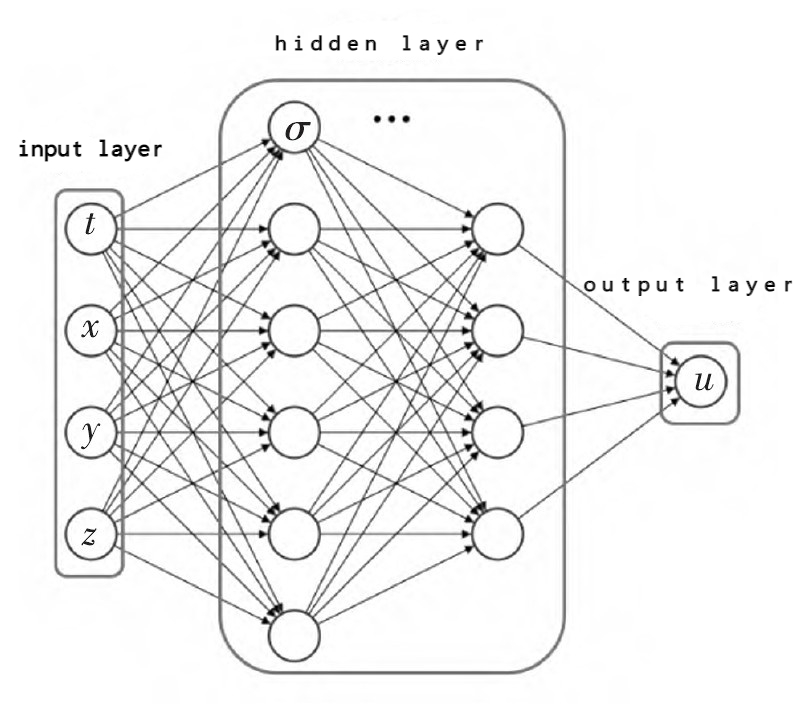
\includegraphics[width=3.5in]{figure/fig1.jpg}
\caption{Schematic diagram of neural network}
\label{fig_1}
\end{figure}

Each neuron in the hidden layer contains an activation function. The activation function is a simple continuous function \cite{ruder2016}, such as the hyperbolic sine function, hyperbolic tangent function, etc. In this paper, the hyperbolic tangent function is selected as the activation function, as shown in Equation (\ref{equ_1}).



\begin{equation}
\tanh{(x)} = \dfrac{e^{x}-e^{-x}}{e^{x}+e^{-x}}
\label{equ_1}
\end{equation}

Usually, activation functions have the same form. For a neuron in the hidden layer, the weighted average of the information transmitted by the neurons in the previous layer, plus paranoia, is used as the input of the neuron, the activation function acts on the input, and the output is passed to the next layer of neurons.

Expressed in the form of a matrix, the information received by the first layer of the hidden layer is shown in Equation (\ref{equ_2}).


\begin{equation}
\mathbf{X_{1}} = \mathbf{W_{1}^{T}} \mathbf{a}
\label{equ_2}
\end{equation}
where:

\begin{equation}
\mathbf{W_{1}^{T}} = \begin{bmatrix}
w_{11} & w_{21} & w_{31} & w_{41} \\
w_{12} & w_{22} & w_{32} & w_{42} \\
w_{13} & w_{23} & w_{33} & w_{43} \\
w_{14} & w_{24} & w_{34} & w_{44} \\
w_{15} & w_{25} & w_{35} & w_{45} \\
w_{16} & w_{26} & w_{36} & w_{46} \\
\end{bmatrix},
\mathbf{a} = \begin{bmatrix}
t \\
x \\
y \\
z \\
\end{bmatrix}
\label{equ_3}
\end{equation}

Equation (\ref{equ_3}) represents the weight coefficient matrix and input information vector of the input layer acting on the first layer of the hidden layer, respectively. Under the action of the activation function, the output information of the neurons in the first layer of the hidden layer is shown in Equation (\ref{equ_4}).


\begin{equation}
\mathbf{Y_{1}} = \sigma \mathbf{(X_{1} + B_{1})} = \sigma(\mathbf{W_{1}^{T} a + B_{1}})
\label{equ_4}
\end{equation}
where $\sigma$ represents the activation function, and $\mathbf{B}_{1}$ represents the bias vector of the neurons in this layer. For the neural network with two hidden layers shown in Fig.\ref{fig_1}, the information is filtered and reaches the output layer as shown in Equation (\ref{equ_5}).

\begin{equation}
\mathbf{u} = \mathbf{W_{3}^{T} Y_{2}} = \mathbf{W_{3}^{T}} \sigma{[\mathbf{W_{2}^{T}} \sigma{(\mathbf{W_{1}^{T}a + \mathbf{B_{1}})}} + \mathbf{B_2}]}
\label{equ_5}
\end{equation}

Where $\mathbf{W_{3}} \in \mathbb{R}^{4 \times 1}$ is the weight coefficient matrix when the second layer of the hidden layer is passed to the output layer. It can be seen that the final output information is a complex non-linear relationship between the input information and a series of weight coefficients and biases. We adjust the weight coefficients and biases so that the non-linear relationship approximates the true solution.

\subsection{Algorithmic Framework}

For the convenience of discussion, without loss of generality, this paper considers the second-order partial differential equation of the following form, as shown in Equation (\ref{equ_6}).

\begin{equation}
f \left (
\begin{aligned}
&\dfrac{\partial^{2} \mathbf{u}}{\partial{t^2}},
\dfrac{\partial^{2} \mathbf{u}}{\partial{x^2}},
\dfrac{\partial^{2} \mathbf{u}}{\partial{y^2}},
\dfrac{\partial^{2} \mathbf{u}}{\partial{z^2}},
\dfrac{\partial^{2} \mathbf{u}}{\partial{x}\partial{t}},
\dfrac{\partial^{2} \mathbf{u}}{\partial{x}\partial{y}},
\dfrac{\partial^{2} \mathbf{u}}{\partial{x}\partial{z}},\\
&\dfrac{\partial^{2} \mathbf{u}}{\partial{y}\partial{t}},
\dfrac{\partial^{2} \mathbf{u}}{\partial{y}\partial{z}},
\dfrac{\partial^{2} \mathbf{u}}{\partial{z}\partial{t}},
\dfrac{\partial \mathbf{u}}{\partial{t}},
\dfrac{\partial \mathbf{u}}{\partial{x}},
\dfrac{\partial \mathbf{u}}{\partial{y}},
\dfrac{\partial \mathbf{u}}{\partial{z}},
C
\end{aligned}
\right ) = 0
\label{equ_6}
\end{equation}

where $C$ represents an arbitrary constant term. Given initial conditions, or boundary conditions, or mixed conditions, the solution of a partial differential equation is uniquely determined. Second, assuming that the solution of the partial differential equation above is approximated using the neural network shown in Fig.\ref{fig_1}, then:



\begin{equation}
\mathbf{u}_{NN} = \mathbf{W_{3}^{T} Y_{2}} = \mathbf{W_{3}^{T}} \sigma{[\mathbf{W_{2}^{T}} \sigma{(\mathbf{W_{1}^{T}a + \mathbf{B_{1}})}} + \mathbf{B_2}]}
\label{equ_7}
\end{equation}

where the meaning of the parameter symbols in the right term is consistent with Section 1.1, $\mathbf{a} = [t,x,y,z ]^{T}$ is the input information vector. On the one hand, since $\mathbf{u}_{NN}$ is not the exact solution of the partial differential equation, when it is substituted into the left end of the original partial differential equation, the result is not equal to zero, but has a margin deviation $\mathbf{R}_{f}$, as shown in Equation (\ref{equ_8}).



\begin{equation}
f \left (
\begin{aligned}
&\frac{\partial^{2} \mathbf{u}_{NN}}{\partial{t^2}},
\dfrac{\partial^{2} \mathbf{u}_{NN}}{\partial{x^2}},
\dfrac{\partial^{2} \mathbf{u}_{NN}}{\partial{y^2}},
\dfrac{\partial^{2} \mathbf{u}_{NN}}{\partial{z^2}},
\dfrac{\partial^{2} \mathbf{u}_{NN}}{\partial{x}\partial{t}},\\
&\dfrac{\partial^{2} \mathbf{u}_{NN}}{\partial{x}\partial{y}},
\dfrac{\partial^{2} \mathbf{u}_{NN}}{\partial{x}\partial{z}},
\dfrac{\partial^{2} \mathbf{u}_{NN}}{\partial{y}\partial{t}},
\dfrac{\partial^{2} \mathbf{u}_{NN}}{\partial{y}\partial{z}},
\dfrac{\partial^{2} \mathbf{u}_{NN}}{\partial{x}\partial{z}},\\
&\dfrac{\partial \mathbf{u}_{NN}}{\partial{t}},
\dfrac{\partial \mathbf{u}_{NN}}{\partial{x}},
\dfrac{\partial \mathbf{u}_{NN}}{\partial{y}},
\dfrac{\partial \mathbf{u}_{NN}}{\partial{z}},
C
\end{aligned}
\right ) = \mathbf{R}_{f}
\label{equ_8}
\end{equation}

It should be pointed out here that in the deep neural network, the partial differentiation of the output information with respect to the input information can be calculated using the automatic differentiation. On the other hand, the residual deviation $\mathbf{R}_{i}$ between the output information corresponding to the initial moment and the initial condition is:


\begin{equation}
(\mathbf{u}_{NN}^{initial} - \mathbf{u}_{0}) = \mathbf{R}_{i}
\label{equ_9}
\end{equation}

where $\mathbf{u}_{NN}^{initial}=\mathbf{W_{3}^{T}} \sigma{[\mathbf{W_{2}^{T}} \sigma{(\mathbf{W_{1}^{T}a + \mathbf{B_{1}})}} + \mathbf{B_2}]},\mathbf{a}_{0}=[0,x,y,z]^{T}$,$u_{0}$ represents the initial condition of the partial differential equation. The residual deviation between the output information on the boundary of the computational domain space and the boundary conditions is $\mathbf{R}_{\Gamma}$:


\begin{equation}
(\mathbf{u}_{NN}^{boundary} - \mathbf{u}_{\Gamma}) = \mathbf{R}_{\Gamma}
\label{equ_10}
\end{equation}

where $\mathbf{u}_{NN}^{boundary}=\mathbf{W_{3}^{T}} \sigma{[\mathbf{W_{2}^{T}} \sigma{(\mathbf{W}_{1}^{T}  \mathbf{a}_{\Gamma} + \mathbf{B}_{1})} + \mathbf{B_2}]},\mathbf{a}_{\Gamma}=[t,x_{\Gamma},y_{\Gamma},z_{\Gamma}]^{T}$,$\mathbf{u}_{\Gamma}$ represents the boundary condition of the partial differential equation. Note that, given the space-time coordinates $[t, x, y, z]^{T}$ of the solution domain, the above three residual deviations can be regarded as functions of the weight coefficient $\mathbf{W}$ and the bias $\mathbf{B}$. Clearly, a good approximation to the solution of partial differential equations should be such that:


\begin{equation}
\begin{aligned}
F_{loss} = 
&\dfrac{1}{N_{t}N_{x}N_{y}N_{z}} \sum_{1}^{N_{t}}  \sum_{1}^{N_{z}} \sum_{1}^{N_{y}} \sum_{1}^{N_{x}} \mathbf{R}_{f}^{2} + \\
&\dfrac{1}{N_{x} N_{y} N_{z}} \sum_{1}^{N_{z}}  \sum_{1}^{N_{y}} \sum_{1}^{N_{x}} \mathbf{R}_{i}^{2} + \\
&\dfrac{1}{N_{t}N_{x_{\Gamma}}N_{y_{\Gamma}}N_{z_{\Gamma}}} \sum_{1}^{N_{t}}  \sum_{1}^{N_{z_{\Gamma}}} \sum_{1}^{N_{y_{\Gamma}}} \sum_{1}^{N_{x_{\Gamma}}} \mathbf{R}_{\Gamma}^{2} 
\end{aligned}
\label{equ_11}
\end{equation}

The value is the smallest under a series of space-time coordinates uniformly distributed over the solution domain. Among them, $N_x$, $N_y$, $N_z$ and $N_t$ are the number of discrete points in the $x,y,z$ and $t$ directions of the computational domain, respectively, and $N_{x_{\Gamma}}$, $N_{y_{\Gamma}}$, $N_{z_{\Gamma}}$ represent the number of discrete points on the $x,y,z$ boundaries of the computational domain, respectively number. The basis for selecting the sum of squares of the deviation margin as the criterion is similar to that of the least squares method. For details, please refer to the relevant literature \cite{kopriva2009}. Equation (\ref{equ_11}) is the minimum objective function based on the deep learning partial differential equation solving algorithm, which can be regarded as a function of a series of weight coefficients $\mathbf{W}$ and bias $\mathbf{B}$, namely:

\begin{equation}
F_{loss} = F(\mathbf{W,B})
\label{equ_12}
\end{equation}

Therefore, the partial differential equation solving problem is finally transformed into an unconstrained optimization problem. Gradient Descent Method and Quasi-Newton algorithm BFGS are common algorithms for solving unconstrained optimization problems\cite{ruder2016}\cite{nocedal1980}. The L-BFGS algorithm used in this paper is an improvement of the BFGS algorithm, which overcomes the disadvantage of high space complexity\cite{nocedal1980}. The algorithm framework is shown in Fig.\ref{fig_2}.



\begin{figure}[!t]
\centering
\includegraphics[width=4in]{figure/fig2.png}
\caption{Algorithm flow chart}
\centering
\label{fig_2}
\end{figure}

\section{Algorithm Verification}

From a mathematical point of view, partial differential equations can be divided into elliptic equations, hyperbolic equations and parabolic equations \cite{logan2014}. In this paper, three examples corresponding to this classification are selected to verify the algorithm.

\subsection{The Initial Value Problem of One-Dimensional Convective Equation}

The one-dimensional convection equation is a typical first-order hyperbolic partial differential equation with the following form:


\begin{equation}
\dfrac{\partial u}{\partial u} + \alpha \dfrac{\partial u}{\partial x} = 0
\label{equ_13}
\end{equation}

where a is a nonzero constant. We know that it is hyperbolic, and its solution is unique given the initial conditions.

Without loss of generality, let $a=-1$ here, and give the following initial conditions:



\begin{equation}
u_{0}(x) = \left\{
\begin{aligned}
&10x+1,-0.1 \leq x \leq 0 \\
&-10x+1,0 \leq x \leq 0.1 \\
&0,otherwise \\
\end{aligned}
\right.
\label{equ_14}
\end{equation}

The initial signal is triangular with a width of 0.2 and the first derivative is discontinuous at $x=0$. In order to test the accuracy of the proposed algorithm, the proposed algorithm and the finite-difference upwind-style algorithm are used to solve the initial value problem of the above hyperbolic partial differential equation. The results at different times are shown in Fig.\ref{fig_3}.


\begin{figure}[!t]
\centering
\subfloat[Upward style]{\includegraphics[width=3.5in]{figure/fig31.png}%
\label{fig_3-1}}
\vfil
\subfloat[Deep learning algorithm]{\includegraphics[width=3.5in]{figure/fig32.png}%
\label{fig_3-2}}
\centering
\caption{Comparison of calculation results using upwind style and deep learning algorithm}
\label{fig_3}
\end{figure}


Ideally, the result of the solution should be a triangular signal shape distributed in different spatial locations at different times. As can be seen from Fig.\ref{fig_3}, due to the introduction of artificial stickiness\cite{LuJinfu2004}, the upwind style "smoothes" the sharp corners of the signal, and the signal strength is also weakened over time. In contrast, the results based on the deep learning algorithm in this paper better preserve the shape and intensity of the initial signal.


\subsection{Boundary Value Problem of Two-Dimensional Laplace Equation}

The two-dimensional Laplace equation is a typical elliptic partial differential equation. Without loss of generality, it is assumed here that it has the following form:


\begin{equation}
\dfrac{\partial^2 u}{\partial{x^2}} + \dfrac{\partial^2{u}}{\partial{u^2}} = 0
\label{equ_15}
\end{equation}

From a physical point of view, this equation describes a steady-state phenomenon, such as the temperature distribution inside a metal plate given the boundary temperature. The boundary conditions of elliptic partial differential equations have the following three formulations: 
\begin{enumerate}
\item[(1)] Dirichlet boundary value condition, that is, the value $U_{1}(x,y)$ of u is given on the given boundary; 
\item[(2)] Neumann boundary value condition, that is, the normal derivative value of u, $\dfrac{\partial u}{\partial n} = U_{2}(x,y)$ is given on the given boundary;
\item[(3)] Robbin boundary value condition, that is, $\dfrac{\partial u}{\partial n} + u = U_{3}(x,y)$.
\end{enumerate}
We take the Dirichlet boundary value condition.Given the following computational domain boundaries and boundary value conditions:


\begin{equation}
\left\{
\begin{aligned}
& 0 \leq x \leq 2,0 \leq y \leq 2 \\
&u(0,y) = 0,u(2,y) = y(2-y) \\
&u(x,0) = 0,u(x,2) = \left\{ 
\begin{aligned}
&2-x,&x > 1\\
&x,&x<1 \\
\end{aligned} 
.\right. \\
\end{aligned}
\right.
\label{equ_16}
\end{equation}
The algorithm in this paper and the five-point difference scheme are used to solve the problem, respectively. The qualitative comparison of the overall distribution cloud map and the quantitative comparison of the results at different locations are shown in Fig.\ref{fig_4}. It can be seen that the algorithm in this paper has comparable accuracy to the five-point difference scheme.




\begin{figure}[!t]
\centering
\subfloat[Qualitative comparison]{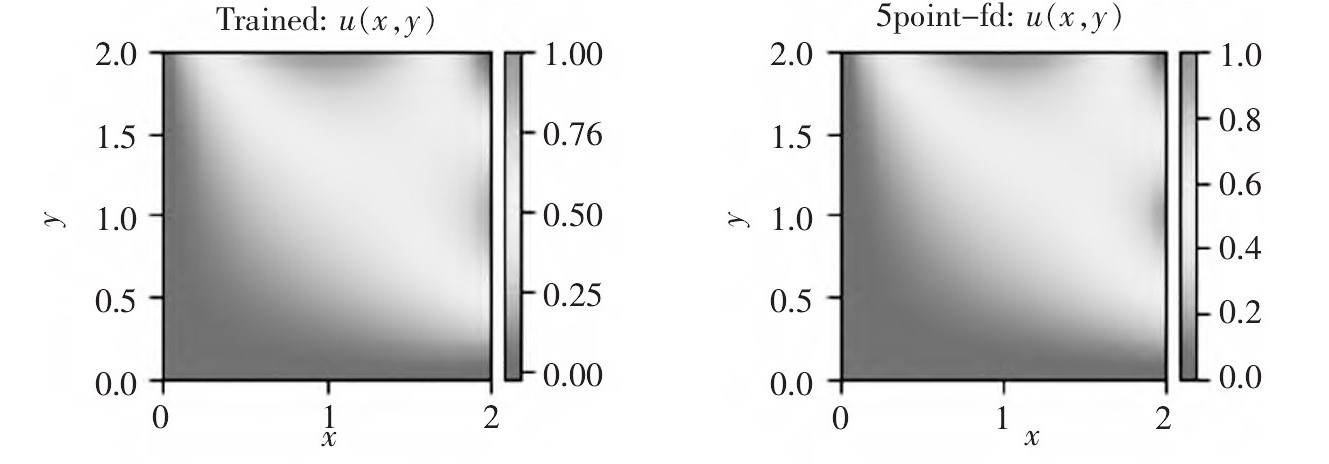
\includegraphics[width=3.5in]{figure/fig41.jpg}%
\label{fig_4-1}}
\vfil
\subfloat[Qualitative comparison]{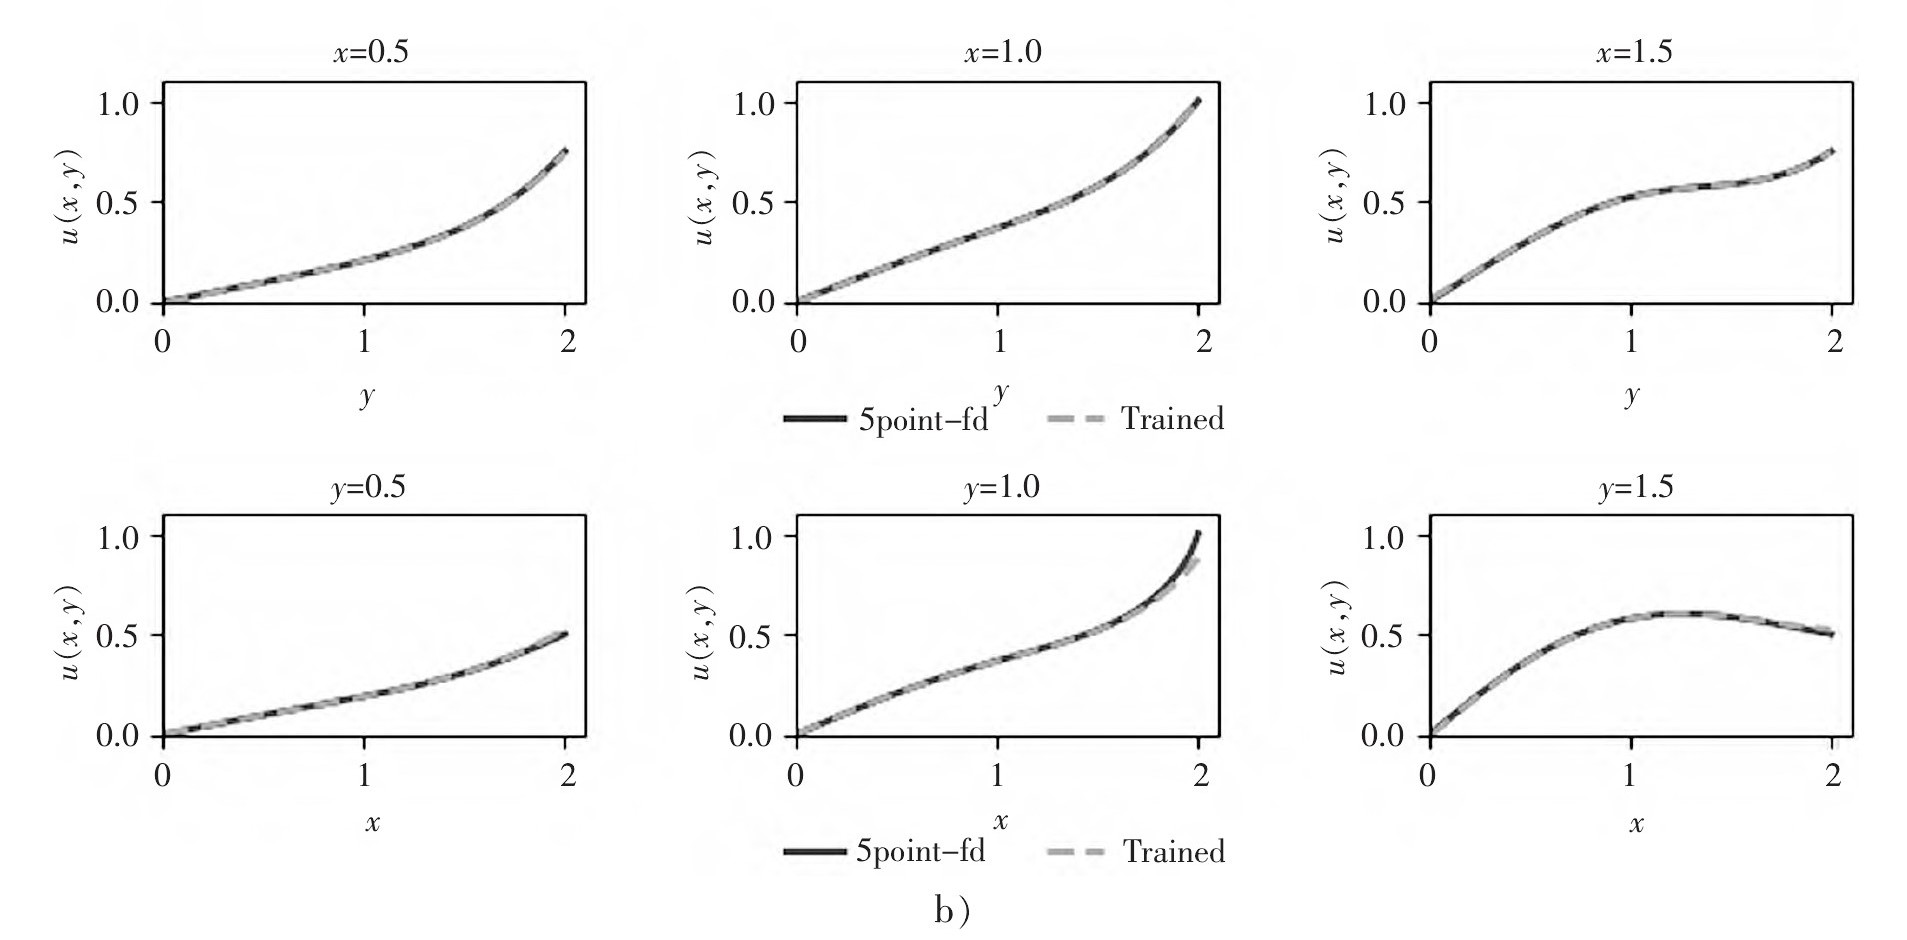
\includegraphics[width=3.5in]{figure/fig42.jpg}%
\label{fig_4-2}}
\caption{Numerical solution results of the two-dimensional Laplace equation}
\label{fig_4}
\end{figure}

Further, this subsection explores the influence of the number and width of the hidden layers (number of neurons in each layer) of the deep neural network on the computational results. For the calculation of the relative error percentage, the result of the five-point difference format is selected as the exact solution. The results are shown in Table\ref{table_1}. It can be seen that for the two-dimensional Laplace equation, as the width of the hidden layer increases, the prediction accuracy of the neural network increases first and then decreases, while with the increase of the number of hidden layers, the prediction accuracy decreases. This shows that when using a neural network to predict the numerical solution of the two-dimensional Laplace equation boundary value problem, using more neurons does not necessarily lead to an improvement in the prediction accuracy.



\begin{table}
\centering
\caption{The relative error percentage of the two-dimensional Laplace equation neural network predicting the numerical solution}
\begin{tabular}{|c|*{3}{c}|}
\hline
\diagbox{Number of Layers}{Width of Layer} & 10 & 20 & 20 \\
\hline
2 & 1.4e-2 & 1.1e-2 & 1.7e-2 \\
4 & 3.1e-2 & 1.6e-2 & 4.1e-2 \\
6 & 3.9e-2 & 3.6e-2 & 4.0e-2 \\
8 & 3.6e-2 & 3.6e-2 & 6.7e-2 \\
\hline

\end{tabular}
\label{table_1}
\end{table}

\subsection{the Initial Boundary Value Problem of One-Dimensional Diffusion Equation}

Diffusion equation is a common parabolic partial differential equation in applications. It has obvious physical background, such as the diffusion process, heat transfer process and wave propagation process between substances with different concentrations. The partial differential equation shown in equation (\ref{equ_17}):

\begin{equation}
\dfrac{\partial u}{\partial t} + \alpha \dfrac{\partial^2{u}}{\partial{x^2}} = 0
\label{equ_17}
\end{equation}

Equation (\ref{equ_17}) is a typical form of the diffusion equation. where a is a non-zero constant. Given initial and boundary conditions, the partial differential equation above has a unique solution.

Choose $a=-1$ and given the following initial and boundary conditions:


\begin{equation}
\left\{
\begin{aligned}
&u(x,0) = \sin{x},0<x<1 \\
&u(0,t) = 0 \\
&u(1,t) = 1 \\
\end{aligned}
\right.
\label{equ_18}
\end{equation}

The algorithm in this paper and the Crank-Nicolson format are used to solve the problem. The overall distribution cloud map predicted by the neural network and the quantitative comparison of the results at different times are shown in Fig.\ref{fig_5}. Among them, Fig.\ref{fig_5-1} is the cloud map of the predicted value of the neural network, and the white line marks the moment of quantitative comparison. It can be seen that the algorithm in this paper has comparable precision with the Crank-Nicolson format.


\begin{figure}[!t]
\centering
\subfloat[Neural network predicted value cloud map]{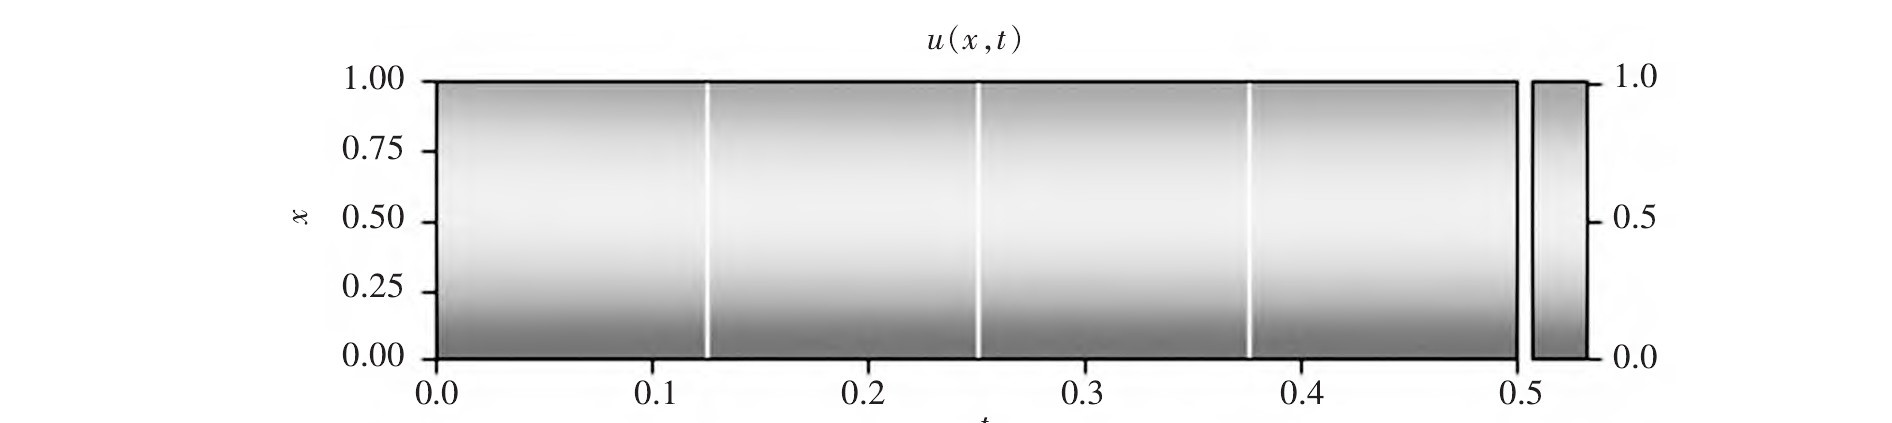
\includegraphics[width=3.5in]{figure/fig51.jpg}%
\label{fig_5-1}}
\vfil
\subfloat[Quantitative comparison]{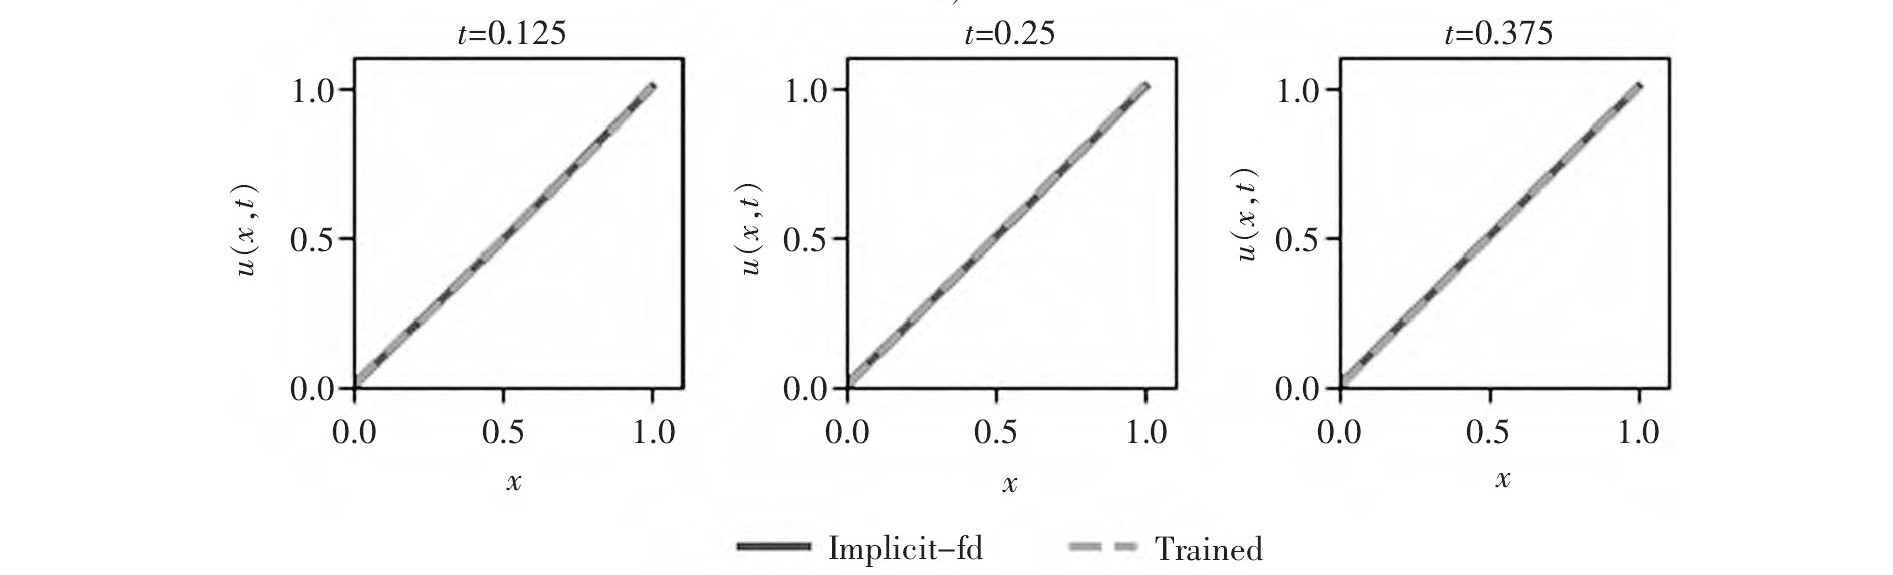
\includegraphics[width=3.5in]{figure/fig52.jpg}%
\label{fig_5-2}}
\caption{Numerical solution results of one-dimensional diffusion equation}
\label{fig_5}
\end{figure}

The relative error is calculated using the Crank-Nicolson format result as the exact solution. It can be seen from the results in Table \ref{table_2} that for the one-dimensional diffusion equation, the influence of the number of layers and depth of the hidden layer of the deep neural network on the prediction accuracy is similar to the results of predicting the two-dimensional Laplace equation.


\begin{table}
\centering
\caption{The relative error percentage of the one-dimensional diffusion equation neural network predicting the numerical solution}

\begin{tabular}{|c|*{3}{c}|}
\hline
\diagbox{Number of Layers}{Width of Layer} & 10 & 20 & 40 \\
\hline
2 & 7.6e-3 & 6.5e-3 & 9.9e-3 \\
4 & 8.5e-3 & 9.5e-3 & 9.2e-3 \\
6 & 9.9e-3 & 9.9e-3 & 1.1e-2 \\
8 & 1.3e-2 & 1.1e-2 & 1.0e-2 \\
\hline
\end{tabular}
\label{table_2}
\end{table}

\section{Conclusion}

We propose a deep learning-based method for solving partial differential equations. For three typical problems of hyperbolic, elliptic and parabolic partial differential equations, the finite difference scheme and the method in this paper are used to solve them. The comparison of the results shows that the algorithm in this paper has better solution accuracy, and it can overcome the disadvantage of artificial stickiness introduced by the upwind style. In addition, the algorithm of this paper does not need special treatment for different types of partial differential equations, that is, the algorithm framework of this paper has wider applicability.

The above advantages of this method do not mean that it can replace the mature traditional methods in engineering applications at present. The reason is that when solving partial differential equations based on deep neural networks, the law of error is not clear. In addition, the use of deep learning methods to solve partial differential equations requires a relatively clear definition of the boundary conditions or initial conditions of the problem, otherwise there may be problems that the boundary cannot be captured or the transient solution is inaccurate. In view of the above two aspects, in the future, we need to conduct in-depth research on the mathematical nature of how deep neural networks converge to the solutions of partial differential equations during the training process.



% An example of a floating figure using the graphicx package.
% Note that \label must occur AFTER (or within) \caption.
% For figures, \caption should occur after the \include.
% Note that IEEEtran v1.7 and later has special internal code that
% is designed to preserve the operation of \label within \caption
% even when the captionsoff option is in effect. However, because
% of issues like this, it may be the safest practice to put all your
% \label just after \caption rather than within \caption{}.
%
% Reminder: the "draftcls" or "draftclsnofoot", not "draft", class
% option should be used if it is desired that the figures are to be
% displayed while in draft mode.
%
%\begin{figure}[!t]
%\centering
%\includegraphics[width=2.5in]{myfigure}
% where an .eps filename suffix will be assumed under latex, 
% and a .pdf suffix will be assumed for pdflatex; or what has been declared
% via \DeclareGraphicsExtensions.
%\caption{Simulation results for the network.}
%\label{fig_sim}
%\end{figure}

% Note that the IEEE typically puts floats only at the top, even when this
% results in a large percentage of a column being occupied by floats.
% However, the Computer Society has been known to put floats at the bottom.


% An example of a double column floating figure using two subfigures.
% (The subfig.sty package must be loaded for this to work.)
% The subfigure \label commands are set within each subfloat command,
% and the \label for the overall figure must come after \caption.
% \hfil is used as a separator to get equal spacing.
% Watch out that the combined width of all the subfigures on a 
% line do not exceed the text width or a line break will occur.
%
%\begin{figure*}[!t]
%\centering
%\subfloat[Case I]{\includegraphics[width=2.5in]{box}%
%\label{fig_first_case}}
%\hfil
%\subfloat[Case II]{\includegraphics[width=2.5in]{box}%
%\label{fig_second_case}}
%\caption{Simulation results for the network.}
%\label{fig_sim}
%\end{figure*}
%
% Note that often IEEE papers with subfigures do not employ subfigure
% captions (using the optional argument to \subfloat[]), but instead will
% reference/describe all of them (a), (b), etc., within the main caption.
% Be aware that for subfig.sty to generate the (a), (b), etc., subfigure
% labels, the optional argument to \subfloat must be present. If a
% subcaption is not desired, just leave its contents blank,
% e.g., \subfloat[].


% An example of a floating table. Note that, for IEEE style tables, the
% \caption command should come BEFORE the table and, given that table
% captions serve much like titles, are usually capitalized except for words
% such as a, an, and, as, at, but, by, for, in, nor, of, on, or, the, to
% and up, which are usually not capitalized unless they are the first or
% last word of the caption. Table text will default to \footnotesize as
% the IEEE normally uses this smaller font for tables.
% The \label must come after \caption as always.
%
%\begin{table}[!t]
%% increase table row spacing, adjust to taste
%\renewcommand{\arraystretch}{1.3}
% if using array.sty, it might be a good idea to tweak the value of
% \extrarowheight as needed to properly center the text within the cells
%\caption{An Example of a Table}
%\label{table_example}
%\centering
%% Some packages, such as MDW tools, offer better commands for making tables
%% than the plain LaTeX2e tabular which is used here.
%\begin{tabular}{|c||c|}
%\hline
%One & Two\\
%\hline
%Three & Four\\
%\hline
%\end{tabular}
%\end{table}


% Note that the IEEE does not put floats in the very first column
% - or typically anywhere on the first page for that matter. Also,
% in-text middle ("here") positioning is typically not used, but it
% is allowed and encouraged for Computer Society conferences (but
% not Computer Society journals). Most IEEE journals/conferences use
% top floats exclusively. 
% Note that, LaTeX2e, unlike IEEE journals/conferences, places
% footnotes above bottom floats. This can be corrected via the
% \fnbelowfloat command of the stfloats package.







% if have a single appendix:
%\appendix[Proof of the Zonklar Equations]
% or
%\appendix  % for no appendix heading
% do not use \section anymore after \appendix, only \section*
% is possibly needed

% use appendices with more than one appendix
% then use \section to start each appendix
% you must declare a \section before using any
% \subsection or using \label (\appendices by itself
% starts a section numbered zero.)
%




% Can use something like this to put references on a page
% by themselves when using endfloat and the captionsoff option.
\ifCLASSOPTIONcaptionsoff
  \newpage
\fi



% trigger a \newpage just before the given reference
% number - used to balance the columns on the last page
% adjust value as needed - may need to be readjusted if
% the document is modified later
%\IEEEtriggeratref{8}
% The "triggered" command can be changed if desired:
%\IEEEtriggercmd{\enlargethispage{-5in}}

% references section

% can use a bibliography generated by BibTeX as a .bbl file
% BibTeX documentation can be easily obtained at:
% http://mirror.ctan.org/biblio/bibtex/contrib/doc/
% The IEEEtran BibTeX style support page is at:
% http://www.michaelshell.org/tex/ieeetran/bibtex/
%\bibliographystyle{IEEEtran}
% argument is your BibTeX string definitions and bibliography database(s)
%\bibliography{IEEEabrv,../bib/paper}
%
% <OR> manually copy in the resultant .bbl file
% set second argument of \begin to the number of references
% (used to reserve space for the reference number labels box)
\begin{thebibliography}{10}

\bibitem{ShiZhongci2000}
石钟慈, \emph{第三种科学方法: 计算机时代的科学计算}.\hskip 1em plus 0.5em minus
  0.4em\relax 清华大学出版社有限公司, 2000.

\bibitem{LuJinfu2004}
陆金甫, 关治, \emph{偏微分方程数值解法}.\hskip 1em plus 0.5em minus
  0.4em\relax 清华大学出版社有限公司, 2004.

\bibitem{logan2014}
J.~D. Logan, \emph{Applied partial differential equations}.\hskip 1em plus
  0.5em minus 0.4em\relax Springer, 2014.

\bibitem{chapra1998}
S.~CHAPRA and R.~P. Canale, ``Numerical methods for engineers: with programing
  and software applications,'' 1998.

\bibitem{kopriva2009}
D.~A. Kopriva, \emph{Implementing spectral methods for partial differential
  equations: Algorithms for scientists and engineers}.\hskip 1em plus 0.5em
  minus 0.4em\relax Springer Science \& Business Media, 2009.

\bibitem{wang2017}
J.-X. Wang, J.~Wu, J.~Ling, G.~Iaccarino, and H.~Xiao, ``A comprehensive
  physics-informed machine learning framework for predictive turbulence
  modeling,'' \emph{arXiv preprint arXiv:1701.07102}, 2017.

\bibitem{duraisamy2015}
K.~Duraisamy, Z.~J. Zhang, and A.~P. Singh, ``New approaches in turbulence and
  transition modeling using data-driven techniques,'' in \emph{53rd AIAA
  Aerospace sciences meeting}, 2015, p. 1284.

\bibitem{ling2016}
J.~Ling, A.~Kurzawski, and J.~Templeton, ``Reynolds averaged turbulence
  modelling using deep neural networks with embedded invariance,''
  \emph{Journal of Fluid Mechanics}, vol. 807, pp. 155--166, 2016.

\bibitem{QiuXipeng2020}
邱锡鹏, \emph{神经网络与深度学习}.\hskip 1em plus 0.5em minus 0.4em\relax
  机械工业出版社, 2020.

\bibitem{ruder2016}
S.~Ruder, ``An overview of gradient descent optimization algorithms,''
  \emph{arXiv preprint arXiv:1609.04747}, 2016.

\bibitem{nocedal1980}
J.~Nocedal, ``Updating quasi-newton matrices with limited storage,''
  \emph{Mathematics of computation}, vol.~35, no. 151, pp. 773--782, 1980.


\end{thebibliography}

% biography section
% 
% If you have an EPS/PDF photo (graphicx package needed) extra braces are
% needed around the contents of the optional argument to biography to prevent
% the LaTeX parser from getting confused when it sees the complicated
% \includegraphics command within an optional argument. (You could create
% your own custom macro containing the \includegraphics command to make things
% simpler here.)
%\begin{IEEEbiography}[{\includegraphics[width=1in,height=1.25in,clip,keepaspectratio]{mshell}}]{Michael Shell}
% or if you just want to reserve a space for a photo:

%\begin{IEEEbiography}{Michael Shell}
%Biography text here.
%\end{IEEEbiography}

% if you will not have a photo at all:
%\begin{IEEEbiographynophoto}{John Doe}
%Biography text here.
%\end{IEEEbiographynophoto}

% insert where needed to balance the two columns on the last page with
% biographies
%\newpage
%
%\begin{IEEEbiographynophoto}{Jane Doe}
%Biography text here.
%\end{IEEEbiographynophoto}

% You can push biographies down or up by placing
% a \vfill before or after them. The appropriate
% use of \vfill depends on what kind of text is
% on the last page and whether or not the columns
% are being equalized.

%\vfill

% Can be used to pull up biographies so that the bottom of the last one
% is flush with the other column.
%\enlargethispage{-5in}



% that's all folks
\end{document}


